\documentclass[11pt, dvipsnames, handout]{beamer}
\newtoggle{full}
\settoggle{full}{true}

\newtoggle{covered}
\settoggle{covered}{false}

\newtoggle{presentable}
\settoggle{presentable}{false}

\newtoggle{dualscreen}
\settoggle{dualscreen}{false}

\usepackage{pgfplots}
%\pgfplotsset{compat = newest}

\usepackage{pgfpages}

\setbeamertemplate{note page}{\pagecolor{yellow!5}\vfill \insertnote \vfill}
\usepackage{collect}
\definecollection{notes}
\newcounter{notestaken}

\usepackage{xpatch}

\usepackage{ulem}

\usepackage[framemethod=tikz]{mdframed}

\usepackage{scalerel}
\usepackage{calc}

%\usepackage{enumitem}
\setlength\fboxsep{.2em}

\usepackage{graphicx} % Allows including images
\usepackage{booktabs} % Allows the use of \toprule, \midrule and \bottomrule in tables

\xpatchcmd{\itemize}
  {\def\makelabel}
  {\setlength{\itemsep}{0.65 em}\def\makelabel}
  {}
  {}


\xpatchcmd{\beamer@enum@}
  {\def\makelabel}
  {\setlength{\itemsep}{0.65 em}\def\makelabel}
  {}
  {}


%\makeatletter
%\renewcommand{\itemize}[1][]{%
%  \beamer@ifempty{#1}{}{\def\beamer@defaultospec{#1}}%
%  \ifnum \@itemdepth >2\relax\@toodeep\else
%    \advance\@itemdepth\@ne
%    \beamer@computepref\@itemdepth% sets \beameritemnestingprefix
%    \usebeamerfont{itemize/enumerate \beameritemnestingprefix body}%
%    \usebeamercolor[fg]{itemize/enumerate \beameritemnestingprefix body}%
%    \usebeamertemplate{itemize/enumerate \beameritemnestingprefix body begin}%
%    \list
%      {\usebeamertemplate{itemize \beameritemnestingprefix item}}
%      {%
%        \setlength\topsep{1em}%NEW
%        \setlength\partopsep{1em}%NEW
%        \setlength\itemsep{1em}%NEW
%        \def\makelabel##1{%
%          {%
%            \hss\llap{{%
%                \usebeamerfont*{itemize \beameritemnestingprefix item}%
%                \usebeamercolor[fg]{itemize \beameritemnestingprefix item}##1}}%
%          }%
%        }%
%      }
%  \fi%
%  \beamer@cramped%
%  \raggedright%
%  \beamer@firstlineitemizeunskip%
%}
%
%
%
%
%
%\makeatother

%\setlist[beamer@enum@]{topsep=1 em}
%\let\origcheckmark\checkmark %screw you dingbat
%\let\checkmark\undefined %screw you dingbat
%\usepackage{dingbat} 
%\let\checkmark\origcheckmark %screw you dingbat






%\usepackage{fontawesome}

\usepackage{mathtools}
\usepackage{etoolbox, calculator}

\usepackage{xcolor}
\usepackage{tikz}
\usetikzlibrary{arrows.meta}
\usetikzlibrary{calc}
\usepackage[nomessages]{fp}
\usepackage{transparent}
\usepackage{accsupp}
%\usepackage{color, xcolor}

%colorblind-friendly palette
%\definecolor{dblue}{RGB}{51,34,136}
\definecolor{lblue}{RGB}{136,204,238}
%\definecolor{green}{RGB}{17,119,51}
\definecolor{tan}{RGB}{221,204,119}
%\definecolor{mauve}{RGB}{204,102,119}

\usepackage{tcolorbox}



\usepackage{xifthen}
\usepackage{nicefrac}
\usepackage{amsmath}
\usepackage{amsthm}
\usepackage{amssymb}
\theoremstyle{definition}
\newtheorem*{define}{Definition}
\newtheorem*{recall}{Recall}


\DeclareMathOperator{\tr}{tr}

\usepackage{multicol}
%\setlength{\columnsep}{1cm}

\usepackage{tablists, amsmath,vwcol, cancel, polynom}
\usetikzlibrary{shapes, patterns, decorations.shapes}
%\usepackage{tikzpeople}
\tikzstyle{vertex}=[shape=circle, minimum size=2mm, inner sep=0, fill]
\tikzstyle{opendot}=[shape=circle, minimum size=2mm, inner sep=0, fill=white, draw]

% common math quick commands
\newcommand{\nicedd}[2]{\nicefrac{\text{d}#1}{\text{d}#2}}
\newcommand{\dd}[2]{\dfrac{\text{d}#1}{\text{d}#2}}
\newcommand{\pd}[2]{\dfrac{\partial #1}{\partial#2}}
\renewcommand{\d}[1]{\text{d}#1}
\newcommand{\ddn}[3]{\dfrac{\text{d}^{#3}#1}{\text{d}#2^{#3}}}
\newcommand{\pdn}[3]{\dfrac{\partial^{#3}#1}{\partial#2^{#3}}}
\newcommand{\p}[0]{^{\prime}}
\newcommand{\pp}[0]{^{\prime\prime}}
\newcommand{\op}[2][\text{L}]{#1 \left[ #2 \right]}

\newcommand{\lap}[1]{\mathcal{L}\left\{#1\right\}}
\newcommand{\lapinv}[1]{\mathcal{L}^{-1}\left\{#1\right\}}
\newcommand{\lapint}[1]{\int_0^\infty e^{-st}#1dt}
\newcommand{\evalat}[2]{\Big|_{#1}^{#2}}

\newcommand{\paren}[1]{ \left( #1 \right)}

\newcommand{\haxis}[4][\normcolor]{\draw[#1, <->] (-#2,0)--(#3,0) node[right]{$#4$}; }


\newcommand{\axis}[4]{\draw[\normcolor, <->] (-#1,0)--(#2,0) 
node[right]{$x$};
\draw[help lines, <->] (0,-#3)--(0,#4) node[above]{$y$};}

\newcommand{\laxis}[6]{\draw[<->] (-#1,0)--(#2,0) 
node[right]{$#5$};
\draw[ <->] (0,-#3)--(0,#4) node[above]{$#6$};}
\newcommand{\xcoord}[2]{
	\draw (#1,.2)--(#1,-.2) node[below]{$#2$};}
\newcommand{\textnode}[3]{
	\draw (#1,#2) node[below]{$#3$};}
	
\newcommand{\nxcoord}[2]{
	\draw (#1,-.2)--(#1,.2) node[above]{$#2$};}
\newcommand{\ycoord}[2]{
	\draw (.2,#1)--(-.2,#1) node[left]{$#2$};}
\newcommand{\nycoord}[2]{
	\draw (-.2,#1)--(.2,#1) node[right]{$#2$};}
\newcommand{\dlim}{\displaystyle\lim}
\newcommand{\dlimx}[1]{\displaystyle\lim_{x \rightarrow #1}}
\newcommand{\stickfig}[2]{
	\draw (#1,#2) arc(-90:270:2mm);
	\draw (#1,#2)--(#1,#2-.5) (#1-.25,#2-.75)--(#1,#2-.5)--(#1+.25,#2-.75) (#1-.2,#2-.2)--(#1+.2,#2-.2);}	

%\newcounter{example}
%\setcounter{example}{1}
%\newcounter{preFrameExample}
%\AtBeginEnvironment{frame}{\setcounter{preFrameExample}{\value{example}}}
%\newcommand{\ex}[1]{
%	 \setcounter{example}{\value{preFrameExample}}
%	 \textcolor{green}{\small\fbox{Example \arabic{example}: #1}}\\[8pt]
%	\stepcounter{example}}
%\newcommand{\exans}[1]{
%	\SUBTRACT{\value{preFrameExample}}{1}{\n}
%	 \textcolor{green}{\small\fbox{Solution \n: #1}}\\[8pt]}
\mode<presentation> {

% The Beamer class comes with a number of default slide themes
% which change the colors and layouts of slides. Below this is a list
% of all the themes, uncomment each in turn to see what they look like.


\usetheme{CambridgeUS}
\usecolortheme[named=black]{structure}


\newcommand{\studentcolor}[0]{ForestGreen}
\newcommand{\normcolor}[0]{NavyBlue}
\newcommand{\alertcolor}{Red}

\setbeamercolor{normal text}{fg=\normcolor}
\setbeamercolor{frametitle}{fg=\normcolor}
\setbeamercolor{section in head/foot}{fg=Black, bg=Gray!20}
\setbeamercolor{subsection in head/foot}{fg=Green!70!Black, bg=Gray!10}
\setbeamercolor{alerted text}{fg=\alertcolor}
\setbeamerfont{alerted text}{series=\bf}
\setbeamertemplate{enumerate items}[default]
\setbeamercolor{enumerate item}{fg=\normcolor}

\setbeamertemplate{footline} % To remove the footer line in all slides uncomment this line
%\setbeamertemplate{footline}[page number] % To replace the footer line in all slides with a simple slide count uncomment this line

\setbeamertemplate{navigation symbols}{} % To remove the navigation symbols from the bottom of all slides uncomment this line
}

\newcommand{\alertbox}[1]{\tcbox[on line, colframe=\alertcolor, colback=White, left=2pt,right=2pt,top=2pt,bottom=2pt]{\usebeamercolor*{normal text}#1}}


\newcommand{\startstu}{\setbeamercolor{normal text}{fg=\studentcolor}\usebeamercolor*{normal text}\setbeamercolor{enumerate item}{fg=\studentcolor}\usebeamercolor*{enumerate item}}
\newcommand{\stopstu}{\setbeamercolor{normal text}{fg=\normcolor}\usebeamercolor*{normal text}\setbeamercolor{enumerate item}{fg=\normcolor}\usebeamercolor*{enumerate item}}

\newcommand{\takenote}[1]{ \begin{collect}{notes}{}{}{}{}  #1  \end{collect}  \addtocounter{notestaken}{1}} %\ifthenelse{\value{notestaken}>0}{\hrulefill\\}{}

\makeatletter
\newcommand{\cover}{\alt{\beamer@makecovered}{\beamer@fakeinvisible}}
\newcommand{\ucover}[1]{\iftoggle{full}{}{\beamer@endcovered}\stopstu#1\startstu\iftoggle{full}{}{\beamer@startcovered}}
\makeatother

\newcommand{\skippause}{ \addtocounter{beamerpauses}{-1}}
\newcommand{\blockpres}{ \skippause \pause }

\newcommand{\studentify}[1]{\startstu #1  \stopstu }
\newcommand{\student}[1]{\iftoggle{full}{ \pause  \studentify{#1} }{\iftoggle{covered}{\studentify{#1}}{\cover{  #1 }}}}
\newcommand{\cstudent}[1]{\student{\begin{center} #1 \end{center}}}
\newcommand{\fullonly}[1]{\iftoggle{full}{ #1}{}}
\newcommand{\presentonly}[1]{\iftoggle{presentable}{ #1}{}}

\usepackage{xparse}
\usepackage{xifthen}

% shortcuts for commonly-used presentation elements
%\NewDocumentCommand{\slide}{o m}
% {\IfValueTF{#1}{\begin{frame}[t]{#1}}{\begin{frame}[t]} #2 \end{frame}}

\newtoggle{iscovered}

\newcommand{\slide}[2][]{%
%\setcounter{notestaken}{0}
\takenote{#2} 
%\ifthenelse{\equal{#1}{}}{\begin{frame}[t]}{\begin{frame}[t]{#1}} #2 \ifthenelse{\value{notestaken}>0}{ \note{\includecollection{notes}}}{} \end{frame}%
\ifthenelse{\equal{#1}{}}{\begin{frame}[t]}{\begin{frame}[t]{#1}} #2 \iftoggle{covered}{\settoggle{iscovered}{true}}{\settoggle{iscovered}{false}}  \note{ \iftoggle{iscovered}{}{\settoggle{covered}{true}} #2 \iftoggle{iscovered}{}{\settoggle{covered}{false}} } \end{frame}%
%\setcounter{notestaken}{0}
}
\newcommand{\defn}[2][]{%
 \setcounter{listcounter}{0}%
\ifthenelse{\equal{#1}{}}{\begin{block}{Definition}}{\begin{block}{#1 :}}%
 #2 \vspace{0.25em} \ifthenelse{\value{listcounter}>0}{\skippause}{} \pause \end{block}%
}



\newcommand{\arr}[2]{\begin{array}{#1}#2\end{array}}
\newcommand{\mat}[2]{\left[\arr{#1}{#2}\right]}
\newcommand{\carray}[1]{\arr{c}{#1}}
\newcommand{\larray}[1]{\arr{l}{#1}}
\newcommand{\rarray}[1]{\arr{r}{#1}}
\newcommand{\colvec}[1]{\mat{c}{#1}}

\newcommand{\itmz}[1]{\addtocounter{listcounter}{1} \begin{itemize}#1 \end{itemize} }
\newcommand{\subitem}[1]{\addtocounter{listcounter}{1} \begin{itemize} \item #1 \end{itemize}}
%
\newcommand{\enum}[1]{\addtocounter{listcounter}{1} \begin{enumerate} #1  \end{enumerate}  }


\newcommand{\algnlbl}[1]{\begin{align}#1  \end{align}} 
\newcommand{\algn}[1]{\begin{align*}#1  \end{align*}} 
\newcommand{\lgn}[1]{ \action<+->{#1} }
\newcommand{\slgn}[1]{\iftoggle{full}{\action<+->{ \startstu #1 \stopstu}}{ \cover{ #1 } } \takenote{$#1$}}

\newcommand{\chckmrk}{\alert{\checkmark}}

\usepackage{pifont}
\newcommand{\xmark}{\alert{\text{\large \ding{55}}}}

\newcommand{\return}[0]{\raisebox{.5ex}{\rotatebox[origin=c]{180}{$\Lsh$}}}
\usepackage{pbox}
%\newcommand{\ex}[1]{\rotatebox[origin=c]{10}{\uline{ex}}:$\;$\pbox[t][][b]{0.9\linewidth}{#1}}
\newcommand{\ex}[1]{\uline{ex}:$\;$\pbox[t][][t]{0.9\linewidth}{#1}}
\newcommand{\eg}[1]{e.g.,$\;$\pbox[t][][t]{0.9\linewidth}{#1}}
\newcommand{\tikzplot}[8][]{%
\begin{tikzpicture}

\begin{scope}[]%
\clip(-#2,-#4) rectangle (#3,#5);%
#8%
\end{scope}%
\laxis{#2}{#3}{#4}{#5}{#6}{#7}%
#1
\end{tikzpicture}%
}


\newcommand{\cancelslide}[1]{%
\begingroup%
\setbeamertemplate{background canvas}{%
\begin{tikzpicture}[remember picture,overlay]%
\draw[line width=2pt,red!60!black] %
  (current page.north west) -- (current page.south east);%
\draw[line width=2pt,red!60!black] %
  (current page.south west) -- (current page.north east);%
\end{tikzpicture}}%
#1%
\endgroup%
}
\renewcommand{\CancelColor}{\color{red}}
\newcommand{\twocols}[3][0.5]{\begin{columns}\begin{column}{#1\textwidth}#2\end{column}\hspace{1em}\vrule{}\hspace{1em}\begin{column}{#1\textwidth}#3\end{column}\end{columns}}

\newcommand{\twomini}[5][1]{\calculatespace \begin{minipage}[t]{\columnwidth}\begin{minipage}[][#1\contentheight][t]{#2\columnwidth}#4\end{minipage}\hfill\begin{minipage}[][#1\contentheight][t]{#3\columnwidth}#5\end{minipage}\end{minipage}}

\newcommand{\threemini}[7][1]{\calculatespace \begin{minipage}[t]{\columnwidth}\begin{minipage}[][#1\contentheight][t]{#2\columnwidth}#5\end{minipage}\hfill\begin{minipage}[][#1\contentheight][t]{#4\columnwidth}#6\end{minipage}\hfill\begin{minipage}[][#1\contentheight][t]{#3\columnwidth}#7\end{minipage}\end{minipage}}


\newcounter{listcounter}
\setcounter{listcounter}{0}



\newif\ifsidebartheme
\sidebarthemetrue

\newdimen\contentheight
\newdimen\contentwidth
\newdimen\contentleft
\newdimen\contentbottom
\makeatletter
\newcommand*{\calculatespace}{%
\contentheight=\paperheight%
\ifx\beamer@frametitle\@empty%
    \setbox\@tempboxa=\box\voidb@x%
  \else%
    \setbox\@tempboxa=\vbox{%
      \vbox{}%
      {\parskip0pt\usebeamertemplate***{frametitle}}%
    }%
    \ifsidebartheme%
      \advance\contentheight by-1em%
    \fi%
  \fi%
\advance\contentheight by-\ht\@tempboxa%
\advance\contentheight by-\dp\@tempboxa%
\advance\contentheight by-\beamer@frametopskip%
\ifbeamer@plainframe%
\contentbottom=0pt%
\else%
\advance\contentheight by-\headheight%
\advance\contentheight by\headdp%
\advance\contentheight by-\footheight%
\advance\contentheight by4pt%
\contentbottom=\footheight%
\advance\contentbottom by-4pt%
\fi%
\contentwidth=\paperwidth%
\ifbeamer@plainframe%
\contentleft=0pt%
\else%
\advance\contentwidth by-\beamer@rightsidebar%
\advance\contentwidth by-\beamer@leftsidebar\relax%
\contentleft=\beamer@leftsidebar%
\fi%
}
\makeatother


\iftoggle{dualscreen}{\setbeameroption{show notes on second screen=right}}{}

\usepackage{circuitikz}

\begin{document}
\section{Lecture 4}
\subsection{Introduction}

\slide[Recall]{

 Linear 1$^{st}$ Order ODEs: $y\p +p(t) y = h(t)$\vspace{.5em}
\itmz{
\item \alert{$h(t)$ is called the inhomogeneity}
\item \alert{$h(t)=0$: Homogeneous ODE}\vspace{.5em}
\item \alert{$h(t)\neq0$: Inhomogeneous ODE}
}\vfill
General Solution:
\algn{ y_{\rm general} &= y_{\rm particular} + y_{\rm homogeneous}\\\student{y_g(t)}&\student{=y_p(t)+Cy_h(t)}}
\small
\itmz{\item Particular part: depends on $h(t)$  \hspace{1em} - \hspace{1em} no arbitrary constants\vfill \student{\subitem{$h(t)=0 \Rightarrow  y_p=0$} }\vfill
\item Homogeneous part: independent of $h(t)$ \hfill - \hfill multiplicative arbitrary constant}

}

\slide[Recall]{

 Linear 1$^{st}$ Order Initial Value Problems (IVPs): \[y\p +p(t) y = h(t); \qquad y(0)=y_0 \]\vspace{.5em}
\vfill
General Solution + Initial Condition:
\algn{y(0)&=y_p(0)+Cy_h(0)\\&=y_0\\
\student{C}&\student{=\frac{y_0-y_p(0)}{y_h(0)}}}
\vfill \student{ 1 Integration Constant + 1 Initial condition = Unique Solution}

}

\slide[ Linear 2$^{nd}$ order ODEs]{
General: \student{$y\pp +p(t)y\p +q(t)y=h(t)$}\\~\\
ICs: \student{$y(0)=y_0,\qquad y\p(0)=v_0$}
\vfill 
For this week (and beyond):
\enum{\item Constant coefficient, homog. \student{\[ ay\pp +by\p+cy=0\]}
\item Constant coefficient, inhomog. \student{\[ ay\pp +by\p+cy=h(t)\]}}
}%end slide


\slide{\huge \vfill \centering Where do 2$^{nd}$ order linear ODEs\\come from? \vfill}
\subsection{Some example systems}
\slide[Spring-dashpot system:]{
\twomini{.4}{.65}{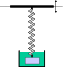
\includegraphics[width=\columnwidth]{images/spring_dashpot.pdf}}{\vfill
$x(t)=$ displacement from rest position\\
$f(t)=$ applied force
\vfill
Newton's 2$^{nd}$ Law:
\algn{ F &= ma\\
 - kx - \beta \dd{x}{t} +f(t) &= m\ddn{x}{t}{2}\\\\ mx\pp+\beta x\p+kx&=f(t)}\vspace*{\fill} }
}


\slide[Torsional motion of a weight on a twisted shaft:]{
\twomini{.32}{.65}{
\includegraphics[width=\columnwidth]{images/twisted_shaft.pdf}}{
\vfill\[ I\ddn{\theta}{t}{2} +c \dd{\theta}{t} + k\theta = T(t)\]\vspace*{\fill}
}
}

\slide[L-R-C series circuits:]{
\twomini{.45}{.55}{
\begin{circuitikz} \draw
       (0,-1.5)   to[vsourcesin, l=\textcolor{black}{$E(t)$}] (0,1.5)
	[black] -- (0.5,1.5)
        to[L, l=$L$, black] (1.5,1.5) -- (2.5,1.5)
        to[C, l=$C$, black] (2.5,0) -- (2.5,-1.5)
        to[R, l=$R$, black] (.5,-1.5) -- (0,-1.5) ;
    \end{circuitikz}
}{\vfill
Q=charge on capacitor\\~\\
$\dd{Q}{t}$=current in circuit\\~\\
$E(t)$ = applied voltage\\
\vfill
Kirchoff's Laws:
\[ L\ddn{Q}{t}{2} +R \dd{Q}{t} + \frac1CQ = E(t)\]\vspace*{\fill}
}
}

\slide[Small oscillations of a pendulum:]{
\twomini{.45}{.55}{\includegraphics[width=\columnwidth]{images/pendulum.pdf}}{
\vfill\[ mL^2\ddn{\theta}{t}{2}=-cL \dd{\theta}{t} -mgL\theta + F(t) \]\vspace*{\fill}
}
}

\slide[Equivalence of Problems]{
These 4 physical systems are modelled identically by:\[Ay\pp+By\p+Cy=D(t)\]
\vfill
Constants have different physical meaning (\& units)
\small\vfill
\begin{tabular}{|>{\centering}m{2cm}|>{\centering}m{2cm}|>{\centering}m{2cm}|>{\centering}m{2cm}|>{\centering}p{2cm}|}
\hline 
\textbf{System} & \textbf{A} & \textbf{B} & \textbf{C} & \textbf{D}\tabularnewline
\hline 
\hline 
\textbf{Spring Dashpot} & Mass & Damping Coeff. & Spring Constant & Applied Force\tabularnewline
\hline 
\textbf{Pendulum} & Mass x (Length)$^{2}$ & Damping x Length & Gravitational Moment & Applied Moment\tabularnewline
\hline 
\textbf{Series Circuit} & Inductance & Resistance & Capacitance$^{-1}$ & Imposed Voltage\tabularnewline
\hline 
\textbf{Twisted Shaft} & Moment of Inertia & Damping & Elastic Shaft Constant & Applied Torque\tabularnewline
\hline 
\end{tabular}

}

\slide[General Linear 2nd Order DE’s]{\vspace{-1em}
\[
\ddn{y}{t}{2} + p(t)\dd{y}{t} +q(t)y=h(t)  
\]

\itmz{\item $h(t)$ represents the "forcing" term, an external influence.
\student{\subitem{$h(t)=0$: solutions tell you the intrinsic behaviour of the system \vfill\subitem{e.g., pull on a spring-mass system, and then let it go} \vfill \item $h(t)\neq0$: solutions tell you the response of the system to forcing \vfill \subitem{e.g., periodically hit a spring-mass system}}}\vfill
\item $p(t)$ and $q(t)$ represent the intrinsic properties of the physical system.
\student{\subitem{Often consant, but not always \subitem{ e.g., an aging spring could be modelled by $q=q(t)$.}}}
}
}
\subsection{Finding solutions - the ansatz method}
\slide{
\ex{$y\pp+3y\p=0$}
\student{We can reduce the order by integrating!
\algn{y\p+3y &= C &
\paren{e^{3t}y}\p &=ce^{3t} \\
e^{3t}y &=\underbrace{\frac{C}{3}}_{c_1}e^{3t} +c_2 &
y &=\textcolor{red}{c_1}+\textcolor{blue}{c_2e^{-3t}}\\
}
This is a special ODE where we can simplify by integrating.\vfill In general, solve using the \uline{ansatz} $y=e^{rt}:$
\algn{y\p &=re^{rt}&
y\pp&=r^2e^{rt}\\
r^2e^{rt}+3re^{rt}&=0&
r(r+3) &=0 \\&&\Rightarrow r=\textcolor{red}{0},\textcolor{blue}{-3}\\
y&=\textcolor{red}{c_1e^0 }+\textcolor{blue}{c_2e^{-3t}} &=\textcolor{red}{c_1 }+\textcolor{blue}{c_2e^{-3t}}
}
}
}%end slide

\slide{
\ex{Solve $y\pp+3y\p=0$ with $y(0)=2$ and $y\p(0)=-2$}
\student{

\algn{ y_g(t) &= c_1+c_2e^{-3t} & y(0) &= c_1 +c_2  = 2\\ y_g\p (t) &= -3c_2e^{3t} & y\p(0) &=-3c_2 = -2\\\\
c_2&=\frac23\\
c_1 +\frac23&=2=\frac63& c_1&=\frac43\\\\
y(t) &= \frac43 + \frac23e^{-3t}
}

}
}%end slide


\slide{
\ex{Find the general solution to $-2y\pp+5y\p+3y=0$}\\~\\
Hint: guess an ansatz $y=e^{rt}$

\student{
\algn{y\p &=re^{rt}&
y\pp&=r^2e^{rt}\\
-2r^2e^{rt}+5re^{rt}+3e^{rt}&=0&
-2r^2+5r+3 &=0 \\ r_{1,2}&=\frac{-5\pm\sqrt{25+24}}{-4} &&=\frac{-5\pm\sqrt{49}}{-4}\\
&=\frac{-5\pm 7}{-4} & &=\frac{2}{-4}, \frac{-12}{-4}\\
&=-\frac12, 3\\
y(t)&=c_1e^{-\frac{t}{2}}+c_2e^{3t}}
}
}%end slide

\slide[Summary]{
\itmz{\item  Linear 2$^{nd}$ order ODEs are useful for modelling many physical systems\vfill
\item  2$^{nd}$ order $\Rightarrow$ 2 Initial Conditions\vfill
\item  Linear 2$^{nd}$ order homogeneous ODEs with constant coefficients \[ ay\pp +by\p+cy=0\]
 Ansatz method:
\enum{\item Guess $y(t)=e^{rt}$ \item Plug guess into the ODE \item Find (up to) 2 values of $r$  }\[y_h=c_1e^{r_1t}+c_2e^{r_2t}\]
}
}



\end{document}